% Created 2012-10-18 Thu 12:04
\documentclass[a4paper]{article}
\usepackage[utf8]{inputenc}
\usepackage{hyperref}
\usepackage{graphicx}
\usepackage{longtable}
\usepackage{float}
\usepackage{pdfpages}
\providecommand{\alert}[1]{\textbf{#1}}

\title{ADA-NCEPH Data Access Procedure}
\author{Ivan Hanigan and Steven McEachern}
\date{\today}
\hypersetup{
  pdfkeywords={},
  pdfsubject={},
  pdfcreator={Emacs Org-mode version 7.8.11}}

\begin{document}

\maketitle

% Org-mode is exporting headings to 3 levels.
\tableofcontents
\hrule
\clearpage
\section{Introduction}
\label{sec-1}

The aim of this document is to describe the procedure for accessing restricted health data through the proposed ANU Secure Data Hub, administered by the ADA and NCEPH.
\section{Getting Access}
\label{sec-2}

  
\subsection{Flow Chart of Steps to Get Access}
\label{sec-2-1}

\begin{figure}[!h]
\centering
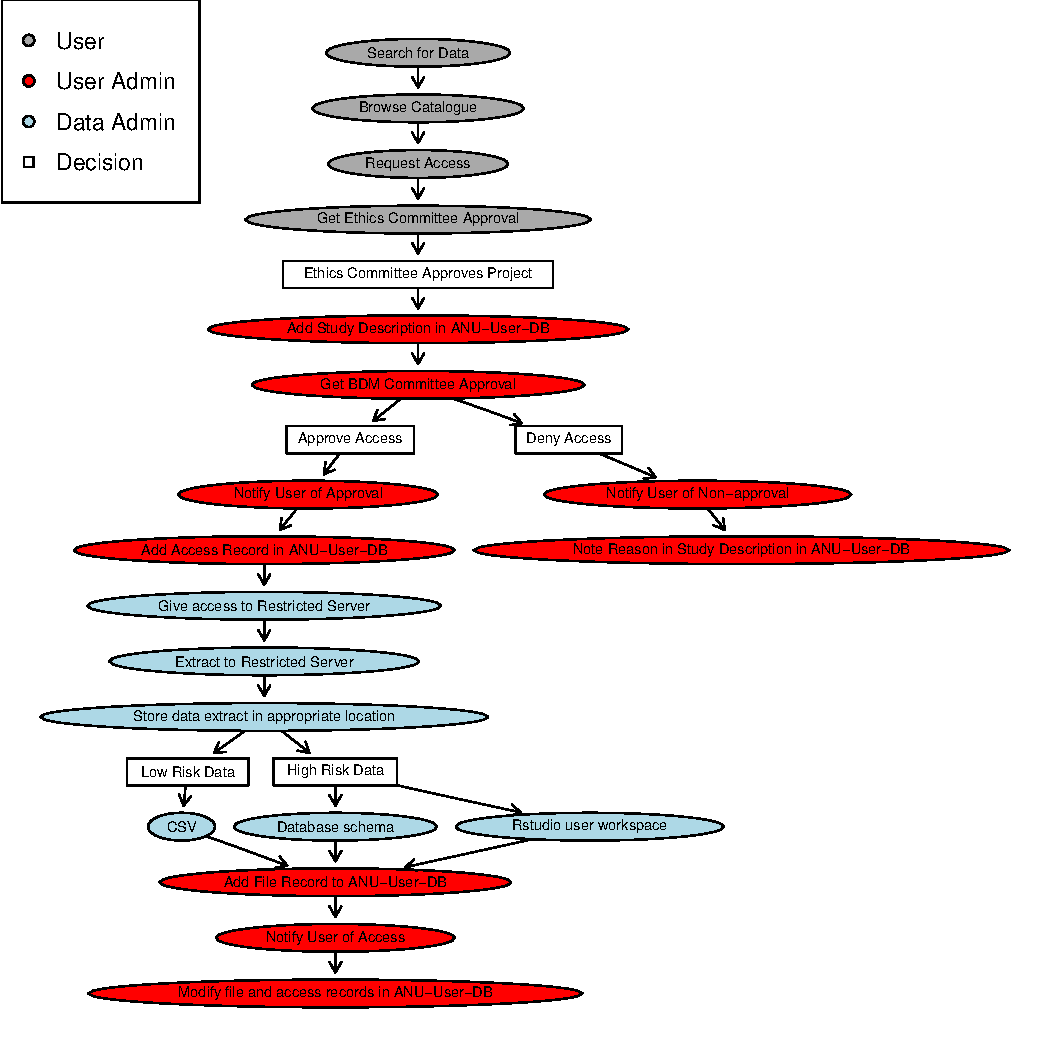
\includegraphics[width=\textwidth]{DataAccessFlowDiagram-GettingAccess.pdf}
\caption{DataAccessFlowDiagram-GettingAccess}
\label{fig:DataAccessFlowDiagram-GettingAccess}
\end{figure}
\clearpage
\section{Managing Access}
\label{sec-3}
\subsection{Query Lists of Projects and Users}
\label{sec-3-1}

This is biannual or annual.
\subsection{Flow Chart of Steps to Manage Access}
\label{sec-3-2}


\begin{figure}[!h]
\centering
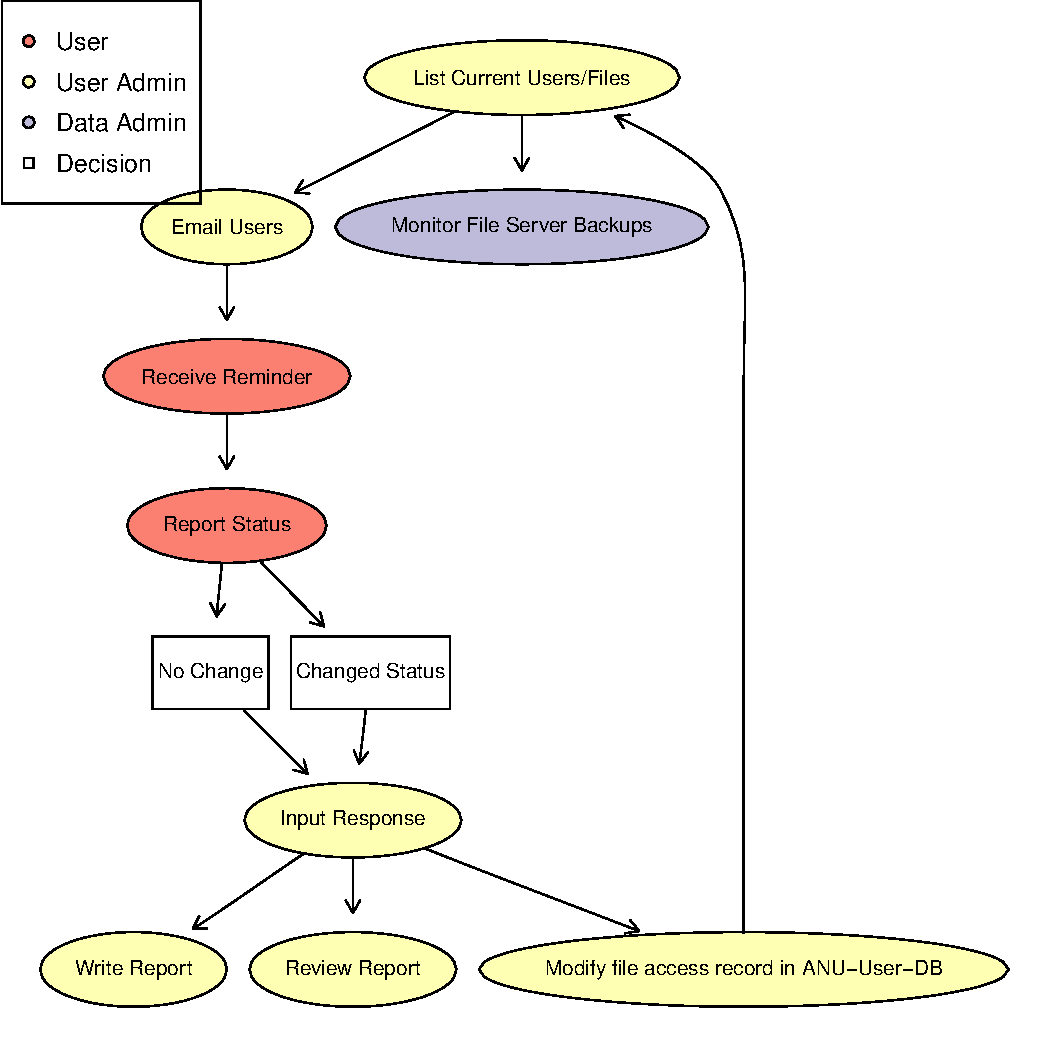
\includegraphics[width=\textwidth]{DataAccessFlowDiagram-ManagingAccess.pdf}
\caption{DataAccessFlowDiagram-ManagingAccess}
\label{fig:DataAccessFlowDiagram-ManagingAccess}
\end{figure}
\clearpage
\section{Ending Access}
\label{sec-4}
\subsection{Query Lists of Registered End Dates}
\label{sec-4-1}
\section{Visualise the Data Access Process}
\label{sec-5}

\end{document}